\documentclass[aspectratio=169]{beamer}
\usetheme{Madrid}
\usecolortheme{default}

% Packages
\usepackage{graphicx}
\usepackage{booktabs}
\usepackage{xcolor}
\usepackage{tikz}
\usetikzlibrary{shapes,arrows,positioning}

% Custom colors
\definecolor{mabscessus}{RGB}{0,191,255}
\definecolor{mtb}{RGB}{255,165,0}
\definecolor{dnacolor}{RGB}{0,0,139}
\definecolor{rosetta}{RGB}{139,69,19}

% Title information
\title[M. abscessus Gyrase Modeling]{Homology Modeling and Molecular Docking of\\
\textit{Mycobacterium abscessus} DNA Gyrase}
\subtitle{RosettaCM Comparative Modeling \& Fluoroquinolone Binding Analysis}
\author{Roy Ahmed}
\institute{Computational Structural Biology}
\date{February 18, 2026}

\begin{document}

%=========================================
% TITLE SLIDE
%=========================================
\begin{frame}
\titlepage
\end{frame}

%=========================================
% OUTLINE
%=========================================
\begin{frame}{Outline}
\tableofcontents
\end{frame}

%=========================================
\section{Introduction}
%=========================================
\begin{frame}{Background \& Motivation}

\begin{columns}
\column{0.5\textwidth}
\textbf{\textit{Mycobacterium abscessus}}
\begin{itemize}
    \item Rapidly growing non-tuberculous mycobacterium
    \item Emerging opportunistic pathogen
    \item Causes pulmonary infections, skin/soft tissue infections
    \item Intrinsic resistance to many antibiotics
    \item Limited treatment options
\end{itemize}

\column{0.5\textwidth}
\textbf{DNA Gyrase as Drug Target}
\begin{itemize}
    \item Essential type II topoisomerase
    \item Introduces negative supercoils in DNA
    \item Required for DNA replication \& transcription
    \item Target of fluoroquinolone antibiotics
    \item No crystal structure available for \textit{M. abscessus}
\end{itemize}
\end{columns}

\vspace{0.3cm}

\begin{block}{Project Goal}
Generate a structural model of \textit{M. abscessus} DNA gyrase using RosettaCM and evaluate fluoroquinolone binding potential
\end{block}

\end{frame}

%=========================================
\section{RosettaCM Methodology}
%=========================================
\begin{frame}{What is RosettaCM?}

\textbf{Rosetta Comparative Modeling (RosettaCM)} -- State-of-the-art homology modeling

\vspace{0.3cm}

\begin{columns}
\column{0.5\textwidth}
\textbf{Key Features}
\begin{itemize}
    \item Multi-template modeling capability
    \item Fragment-based loop sampling
    \item Physics-based energy function
    \item All-atom refinement
    \item Handles insertions/deletions
    \item Produces diverse model ensemble
\end{itemize}

\column{0.5\textwidth}
\textbf{Advantages over Traditional Methods}
\begin{itemize}
    \item Better loop modeling accuracy
    \item Rosetta energy minimization
    \item Can model regions without template
    \item Incorporates evolutionary constraints
    \item Validated in CASP competitions
\end{itemize}
\end{columns}

\vspace{0.3cm}

\begin{alertblock}{Why RosettaCM for This Project?}
DNA gyrase is a large multi-domain complex requiring accurate modeling of protein-DNA interface and loop regions -- RosettaCM excels at these challenges
\end{alertblock}

\end{frame}

%=========================================
\begin{frame}{RosettaCM Pipeline Overview}

\begin{center}
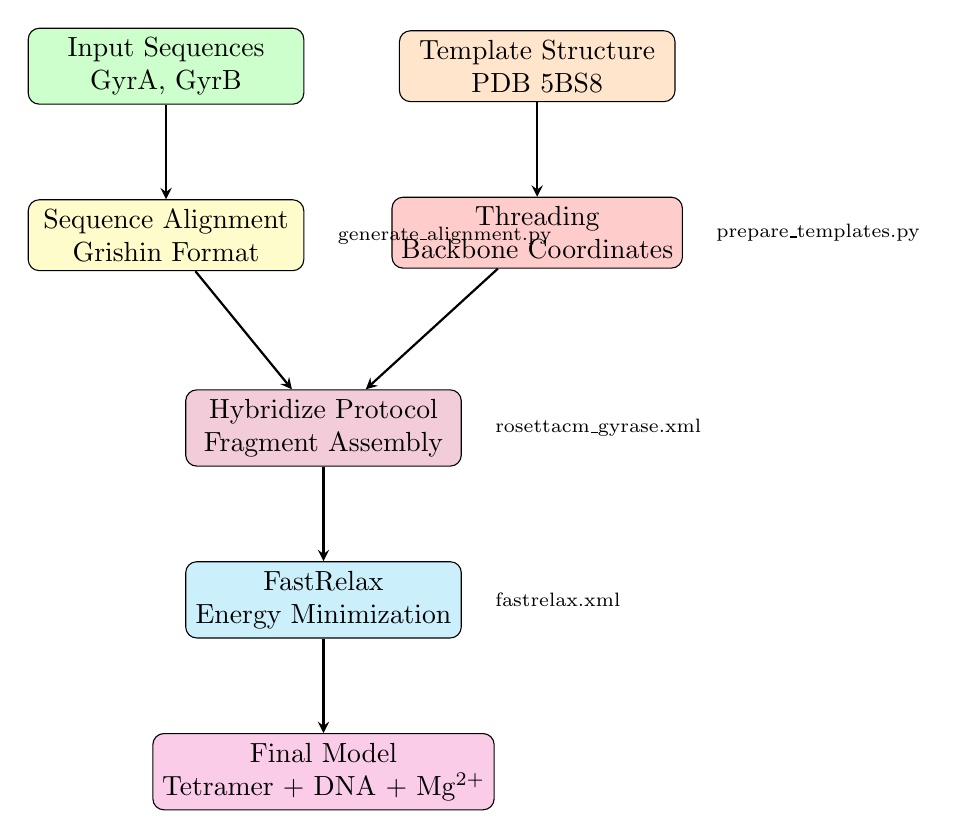
\begin{tikzpicture}[
    node distance=1.2cm,
    box/.style={rectangle, draw, rounded corners, fill=blue!20, minimum width=3.5cm, minimum height=0.8cm, align=center},
    arrow/.style={->, thick, >=stealth}
]

% Nodes
\node[box, fill=green!20] (input) {Input Sequences\\GyrA, GyrB};
\node[box, fill=orange!20, right=of input] (template) {Template Structure\\PDB 5BS8};
\node[box, fill=yellow!20, below=of input] (align) {Sequence Alignment\\Grishin Format};
\node[box, fill=red!20, below=of template] (thread) {Threading\\Backbone Coordinates};
\node[box, fill=purple!20, below=1.5cm of align, xshift=2cm] (hybrid) {Hybridize Protocol\\Fragment Assembly};
\node[box, fill=cyan!20, below=of hybrid] (relax) {FastRelax\\Energy Minimization};
\node[box, fill=magenta!20, below=of relax] (output) {Final Model\\Tetramer + DNA + Mg$^{2+}$};

% Arrows
\draw[arrow] (input) -- (align);
\draw[arrow] (template) -- (thread);
\draw[arrow] (align) -- (hybrid);
\draw[arrow] (thread) -- (hybrid);
\draw[arrow] (hybrid) -- (relax);
\draw[arrow] (relax) -- (output);

% Labels
\node[right=0.3cm of align, font=\scriptsize] {generate\_alignment.py};
\node[right=0.3cm of thread, font=\scriptsize] {prepare\_templates.py};
\node[right=0.3cm of hybrid, font=\scriptsize] {rosettacm\_gyrase.xml};
\node[right=0.3cm of relax, font=\scriptsize] {fastrelax.xml};

\end{tikzpicture}
\end{center}

\end{frame}

%=========================================
\begin{frame}{Step 1: Sequence Alignment}

\textbf{Aligning \textit{M. abscessus} sequences to \textit{M. tuberculosis} template}

\vspace{0.3cm}

\begin{columns}
\column{0.5\textwidth}
\textbf{Input Sequences}
\begin{itemize}
    \item \textbf{GyrA}: UniProt B1ME58
    \begin{itemize}
        \item 838 amino acids
        \item DNA breakage-reunion domain
        \item Contains QRDR (res 80-95)
    \end{itemize}
    \item \textbf{GyrB}: UniProt B1ME45
    \begin{itemize}
        \item 714 amino acids
        \item ATPase domain
        \item TOPRIM domain
    \end{itemize}
\end{itemize}

\column{0.5\textwidth}
\textbf{Grishin Alignment Format}
\begin{itemize}
    \item Required by RosettaCM
    \item Maps query $\rightarrow$ template residues
    \item Handles gaps and insertions
    \item Example:
\end{itemize}
\vspace{0.2cm}
\footnotesize
\texttt{## B1ME58\_GyrA 5bs8\_chainA.pdb}\\
\texttt{scores\_from\_program: 0}\\
\texttt{0 MSDLAREIT...}\\
\texttt{0 MSDLAREIT...}
\end{columns}

\vspace{0.3cm}

\begin{block}{Script Used}
\texttt{scripts/generate\_alignment.py} -- Creates Grishin format alignments
\end{block}

\end{frame}

%=========================================
\begin{frame}{Step 2: Template Preparation}

\textbf{Processing PDB 5BS8 (\textit{M. tuberculosis} DNA Gyrase)}

\vspace{0.3cm}

\begin{columns}
\column{0.55\textwidth}
\textbf{Template Structure Contents}
\begin{itemize}
    \item \textbf{Chain A, C}: GyrA subunits (DNA binding)
    \item \textbf{Chain B, D}: GyrB subunits (ATPase)
    \item \textbf{Chain E, F}: DNA strands (20+ bp)
    \item \textbf{MG}: Magnesium ions (catalytic)
    \item Resolution: 2.5-3.0 \AA
\end{itemize}

\vspace{0.2cm}

\textbf{Preparation Steps}
\begin{enumerate}
    \item Extract individual chains
    \item Fix missing atoms (REDUCE)
    \item Renumber residues if needed
    \item Clean HETATM records
\end{enumerate}

\column{0.45\textwidth}
\textbf{Files Generated}
\begin{itemize}
    \item \texttt{5bs8\_chainA\_fixed.pdb}
    \item \texttt{5bs8\_chainB\_fixed.pdb}
    \item \texttt{5bs8\_dna\_mg.pdb}
    \item \texttt{5bs8\_protein\_only.pdb}
\end{itemize}

\vspace{0.3cm}

\begin{block}{Script Used}
\texttt{scripts/prepare\_templates.py}
\end{block}
\end{columns}

\end{frame}

%=========================================
\begin{frame}{Step 3: RosettaCM Threading (Hybridize Protocol)}

\textbf{Core of RosettaCM -- Threading sequence onto template backbone}

\vspace{0.2cm}

\begin{columns}
\column{0.55\textwidth}
\textbf{Hybridize Protocol}
\begin{enumerate}
    \item \textbf{Stage 1}: Centroid-level assembly
    \begin{itemize}
        \item Copy backbone from template
        \item Monte Carlo fragment insertion
        \item Build unaligned regions de novo
    \end{itemize}
    \item \textbf{Stage 2}: Full-atom refinement
    \begin{itemize}
        \item Add side chains (rotamer packing)
        \item Minimize clashes
        \item Optimize H-bonds
    \end{itemize}
    \item \textbf{Stage 3}: Cartesian minimization
    \begin{itemize}
        \item Fine-tune geometry
        \item Relieve strain
    \end{itemize}
\end{enumerate}

\column{0.45\textwidth}
\textbf{XML Protocol}
\footnotesize
\begin{verbatim}
<Hybridize name="hybridize"
  stage1_scorefxn="stage1"
  stage2_scorefxn="stage2"
  fa_scorefxn="talaris2014">
  <Template pdb="template.pdb"
    cst_file="AUTO"
    weight="1.0"/>
</Hybridize>
\end{verbatim}
\normalsize

\vspace{0.2cm}

\begin{alertblock}{Key Parameter}
\texttt{-nstruct 10} -- Generate 10 models, select best by energy
\end{alertblock}
\end{columns}

\end{frame}

%=========================================
\begin{frame}{Step 4: Tetramer Assembly}

\textbf{Building the complete GyrA$_2$GyrB$_2$ tetramer}

\vspace{0.3cm}

\begin{columns}
\column{0.5\textwidth}
\textbf{Assembly Process}
\begin{enumerate}
    \item Thread GyrA onto chains A, C
    \item Thread GyrB onto chains B, D
    \item Apply symmetry operations
    \item Merge into single PDB file
    \item Add DNA from template (conserved)
    \item Add Mg$^{2+}$ ions at catalytic sites
\end{enumerate}

\vspace{0.2cm}

\textbf{Interface Optimization}
\begin{itemize}
    \item GyrA-GyrA dimer interface
    \item GyrA-GyrB heterodimer interface
    \item Protein-DNA contacts
\end{itemize}

\column{0.5\textwidth}
\begin{center}
\textbf{Tetramer Architecture}
\vspace{0.3cm}

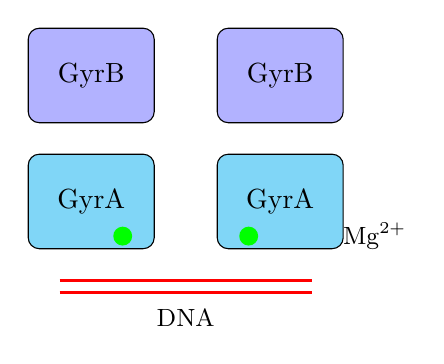
\begin{tikzpicture}[scale=0.8]
% GyrA subunits
\draw[fill=cyan!50, rounded corners] (0,0) rectangle (2,1.5);
\node at (1, 0.75) {GyrA};
\draw[fill=cyan!50, rounded corners] (3,0) rectangle (5,1.5);
\node at (4, 0.75) {GyrA};

% GyrB subunits
\draw[fill=blue!30, rounded corners] (0,2) rectangle (2,3.5);
\node at (1, 2.75) {GyrB};
\draw[fill=blue!30, rounded corners] (3,2) rectangle (5,3.5);
\node at (4, 2.75) {GyrB};

% DNA
\draw[very thick, red] (0.5,-0.5) -- (4.5,-0.5);
\draw[very thick, red] (0.5,-0.7) -- (4.5,-0.7);
\node at (2.5, -1.1) {\small DNA};

% Mg ions
\fill[green] (1.5, 0.2) circle (0.15);
\fill[green] (3.5, 0.2) circle (0.15);
\node at (5.5, 0.2) {\small Mg$^{2+}$};
\end{tikzpicture}
\end{center}
\end{columns}

\vspace{0.2cm}

\begin{block}{Script Used}
\texttt{scripts/assemble\_tetramer.py}
\end{block}

\end{frame}

%=========================================
\begin{frame}{Step 5: FastRelax Refinement}

\textbf{Energy minimization to optimize model geometry}

\vspace{0.3cm}

\begin{columns}
\column{0.55\textwidth}
\textbf{FastRelax Protocol}
\begin{itemize}
    \item Iterative minimization + repacking
    \item 5 cycles of refinement
    \item Ramping repulsive term (fa\_rep)
    \item Allows escape from local minima
\end{itemize}

\vspace{0.2cm}

\textbf{Energy Terms Optimized}
\begin{itemize}
    \item \texttt{fa\_atr}: Attractive van der Waals
    \item \texttt{fa\_rep}: Repulsive van der Waals
    \item \texttt{fa\_sol}: Solvation energy
    \item \texttt{hbond\_*}: Hydrogen bonds
    \item \texttt{rama}: Ramachandran preferences
    \item \texttt{omega}: Peptide bond planarity
\end{itemize}

\column{0.45\textwidth}
\textbf{XML Protocol}
\footnotesize
\begin{verbatim}
<FastRelax name="relax"
  scorefxn="ref2015"
  repeats="5">
  <MoveMap>
    <Chain number="1" chi="1"
      bb="1"/>
  </MoveMap>
</FastRelax>
\end{verbatim}
\normalsize

\vspace{0.3cm}

\begin{block}{Output}
\texttt{output/relaxed/*.pdb}\\
Energy-minimized structures
\end{block}
\end{columns}

\end{frame}

%=========================================
\begin{frame}{RosettaCM XML Configuration File}

\textbf{Key sections of \texttt{xml/rosettacm\_gyrase.xml}}

\vspace{0.2cm}

\footnotesize
\begin{verbatim}
<ROSETTASCRIPTS>
  <SCOREFXNS>
    <ScoreFunction name="stage1" weights="score3"/>
    <ScoreFunction name="stage2" weights="score4_smooth"/>
    <ScoreFunction name="fullatom" weights="ref2015"/>
  </SCOREFXNS>

  <MOVERS>
    <Hybridize name="hybridize"
      stage1_scorefxn="stage1" stage2_scorefxn="stage2"
      fa_scorefxn="fullatom" batch="true">
      <Template pdb="%%template%%" cst_file="AUTO" weight="1.0"/>
    </Hybridize>
    <FastRelax name="relax" scorefxn="fullatom" repeats="5"/>
  </MOVERS>

  <PROTOCOLS>
    <Add mover="hybridize"/>
    <Add mover="relax"/>
  </PROTOCOLS>
</ROSETTASCRIPTS>
\end{verbatim}
\normalsize

\end{frame}

%=========================================
\section{Results}
%=========================================
\begin{frame}{Model Quality Assessment}

\textbf{Structural Alignment: Model vs Template}

\vspace{0.3cm}

\begin{columns}
\column{0.5\textwidth}
\begin{table}
\centering
\begin{tabular}{lcc}
\toprule
\textbf{Subunit} & \textbf{RMSD (\AA)} & \textbf{Quality} \\
\midrule
GyrA (838 aa) & 1.22 & Good \\
GyrB (714 aa) & 0.75 & Excellent \\
\midrule
Overall & $<$1.5 & High quality \\
\bottomrule
\end{tabular}
\caption{C$\alpha$ RMSD values}
\end{table}

\textbf{Interpretation}
\begin{itemize}
    \item RMSD $<$ 2\AA\ = reliable model
    \item Core domains highly conserved
    \item QRDR binding site well-modeled
\end{itemize}

\column{0.5\textwidth}
\textbf{Disjoint Regions Identified}
\begin{itemize}
    \item GyrA: residues 17-19 (3 aa, minor)
    \item GyrB: residues 559-620 (62 aa, major loop)
    \item Located away from active site
    \item Can be refined with loop modeling
\end{itemize}

\vspace{0.3cm}

\textbf{Visualization Colors}
\begin{itemize}
    \item \textcolor{cyan}{Cyan}: \textit{M. abscessus} model
    \item \textcolor{orange}{Orange}: \textit{M. tuberculosis} template
    \item \textcolor{red}{Red}: Disjoint loops
\end{itemize}
\end{columns}

\end{frame}

%=========================================
\begin{frame}{Molecular Docking Results}

\textbf{Fluoroquinolone Binding: \textit{M. abscessus} vs \textit{M. tuberculosis}}

\vspace{0.3cm}

\begin{table}
\centering
\large
\begin{tabular}{lccc}
\toprule
\textbf{Ligand} & \textbf{\textit{M. abscessus}} & \textbf{\textit{M. tuberculosis}} & \textbf{$\Delta$G} \\
\midrule
\rowcolor{yellow!30} Moxifloxacin & \textbf{-7.91} kcal/mol & -7.24 kcal/mol & \textbf{-0.67} \\
\rowcolor{magenta!20} Levofloxacin & -7.65 kcal/mol & -7.31 kcal/mol & -0.34 \\
\rowcolor{green!20} Ciprofloxacin & -7.36 kcal/mol & -7.27 kcal/mol & -0.09 \\
\bottomrule
\end{tabular}
\end{table}

\vspace{0.3cm}

\begin{columns}
\column{0.5\textwidth}
\begin{alertblock}{Key Finding}
All fluoroquinolones show \textbf{stronger binding} to the \textit{M. abscessus} model
\end{alertblock}

\column{0.5\textwidth}
\textbf{Best Candidate}: Moxifloxacin
\begin{itemize}
    \item Strongest affinity (-7.91 kcal/mol)
    \item 0.67 kcal/mol improvement
    \item Already used clinically
\end{itemize}
\end{columns}

\end{frame}

%=========================================
\section{Conclusions}
%=========================================
\begin{frame}{Summary \& Conclusions}

\begin{columns}
\column{0.55\textwidth}
\textbf{What We Accomplished}
\begin{enumerate}
    \item Built RosettaCM pipeline for gyrase modeling
    \item Generated high-quality \textit{M. abscessus} model
    \item Validated structure (RMSD $<$ 1.5 \AA)
    \item Identified QRDR binding site
    \item Docked 3 fluoroquinolone antibiotics
    \item Compared binding to template species
    \item Created visualization movie (8 scenes)
\end{enumerate}

\column{0.45\textwidth}
\begin{block}{Clinical Implications}
\begin{itemize}
    \item Fluoroquinolones bind favorably
    \item \textbf{Moxifloxacin} = best candidate
    \item QRDR conserved $\rightarrow$ drug sensitive
    \item Model enables drug design
\end{itemize}
\end{block}

\vspace{0.2cm}

\textbf{Files Generated}
\begin{itemize}
    \item \texttt{mabs\_gyrase\_tetramer\_dna\_mg.pdb}
    \item \texttt{docked\_*.pdbqt}
    \item \texttt{create\_movie.pml}
\end{itemize}
\end{columns}

\end{frame}

%=========================================
\begin{frame}{Future Directions}

\begin{columns}
\column{0.5\textwidth}
\textbf{Computational Extensions}
\begin{itemize}
    \item Loop refinement (GyrB 559-620)
    \begin{itemize}
        \item Rosetta KIC protocol
        \item NGK loop modeling
    \end{itemize}
    \item Molecular dynamics simulations
    \begin{itemize}
        \item Binding stability (100 ns)
        \item MM-PBSA free energy
    \end{itemize}
    \item Resistance mutation analysis
    \begin{itemize}
        \item Ser83Leu, Asp87Asn
        \item $\Delta\Delta$G calculations
    \end{itemize}
    \item Virtual screening campaigns
\end{itemize}

\column{0.5\textwidth}
\textbf{Experimental Validation}
\begin{itemize}
    \item Enzyme inhibition assays (IC$_{50}$)
    \item MIC determination
    \item X-ray crystallography
    \item Cryo-EM structure
\end{itemize}

\vspace{0.3cm}

\begin{block}{Long-term Goal}
Structure-based drug design for novel anti-\textit{M. abscessus} agents
\end{block}
\end{columns}

\end{frame}

%=========================================
\begin{frame}{Acknowledgments}

\textbf{Software \& Tools}
\begin{itemize}
    \item \textbf{Rosetta}: RosettaCM, FastRelax, Hybridize protocol
    \item \textbf{AutoDock Vina}: Molecular docking
    \item \textbf{PyMOL}: Visualization and movie creation
    \item \textbf{OpenBabel}: File format conversion
\end{itemize}

\vspace{0.3cm}

\textbf{Data Sources}
\begin{itemize}
    \item Template: PDB 5BS8 (\textit{M. tuberculosis} gyrase-DNA complex)
    \item Reference: PDB 5CDQ (gyrase with moxifloxacin)
    \item Sequences: UniProt B1ME45 (GyrB), B1ME58 (GyrA)
    \item Ligands: PubChem (moxifloxacin, ciprofloxacin, levofloxacin)
\end{itemize}

\vspace{0.5cm}

\begin{center}
\Large\textbf{Thank You!}\\
\vspace{0.2cm}
\normalsize Questions?
\end{center}

\end{frame}

\end{document}
